\section{Related Work}
  \citeauthor{zeiler_adaptive_2011} first attempted to use `deconvolution' to
  improve their learning \cite{zeiler_adaptive_2011}, then later for purely
  visualization purposes \cite{zeiler_visualizing_2014}. Their method
  involves monitoring network nodes, seeing what input image causes the largest
  activity and mapping activations at different layers of the network back to the pixel
  space using meta-information from these images.

  \autoref{fig:ch4:deconv_feature} shows the block diagram for how deconvolution is
  done. They invert a convolutional layer by taking the 2D transpose of each
  slice of the filter. Inverting a ReLU is done by simply applying a ReLU again
  (ensuring only positive values can flow back through the network).
  Inverting a max pooling step is a little trickier, as max pooling is quite a lossy
  operation. \citeauthor{zeiler_adaptive_2011} get around this by saving extra
  information on the forward pass of the model --- switches that store the
  location of the input that caused the maximum value. This way, on the
  backwards pass, it is trivial to store activations to the right position in
  the larger feature map. The positions that did not contribute to
  the max pooling operation remain as zero on the backwards pass. This is shown
  in the bottom half of \autoref{fig:ch4:deconv_feature}.

  \begin{figure}
    \centering
      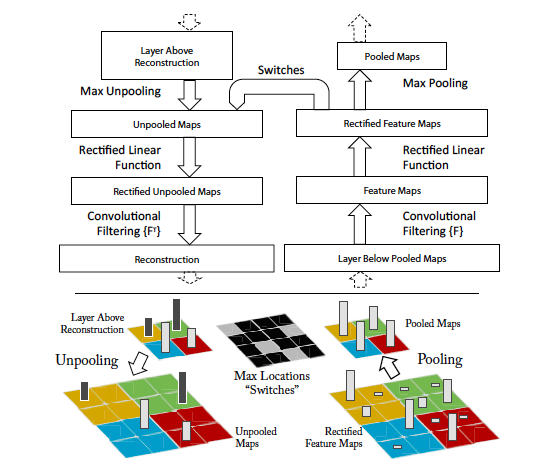
\includegraphics[width=0.7\textwidth]{\imgpath/deconvnet.png}
      \mycaption{Deconvolution network block diagram}{Switches
              are saved alongside pooled features, and the filters
              used for deconvolution are the transpose of the filters used for
              a forward pass. Taken from \cite{zeiler_visualizing_2014}.}
      \label{fig:ch4:deconv_feature}
  \end{figure}

  % \begin{figure}
    % \centering
      % \includegraphics[width=\textwidth]{\imgpath/deconv_switches.png}
      % \caption{Unpooling operation in a deconvnet}{On the forward pass, the
              % locations of the maximum values are stored (the centre map with
              % grey squares). This is then used on the backwards pass to put
              % values at the correct location. Figure taken from \citep{zeiler_visualizing_2014}.}
      % \label{fig:ch4:deconv_switches}
  % \end{figure}
  \citeauthor{mahendran_understanding_2015} take a slightly different route on
  deconvolution networks \cite{mahendran_understanding_2015}. They do not
  store this extra information but instead define a cost function to maximize.
  This results in visualization images that look very surreal, and can be
  quite different from the input.

  In \cite{springenberg_striving_2015}, the authors design an \emph{all convolutional} model,
  where they replace the max pooling layers commonly seen in CNNs with a
  convolutional block with stride 2, i.e.\ a convolution followed by decimation.
  They did this by first adding an extra convolutional layer before the max
  pooling layers, then taking away the max pooling and adding decimation after
  convolution, noting that removing the max pooling had little effect.

  The benefit of this is that they can now reconstruct images as Zeiler and
  Fergus did, but without having to save switches from the max pooling
  operation. Additionally, they modify the handling of the ReLU in the
  backwards pass to combine the regular backpropagation action and the ReLU
  action from deconvolution. They call this `guided backprop'.

  Another interrogation tool commonly used is occlusion or perturbation.
  In \cite{zeiler_visualizing_2014}, \citeauthor{zeiler_visualizing_2014} occlude regions in the
  input image and measure the impact this has on classification score. In
  \cite{fong_interpretable_2017}, \citeauthor{fong_interpretable_2017} use
  gradients to find the minimal mask to apply to the input image that causes
  misclassification.
  % \autoref{fig:ch4:deconv_slices} gives a more detailed view of how the
  % deconvolution works for convolutional layers.
  % \begin{figure}
    % \centering
      % \includegraphics[width=\textwidth]{\imgpath/deconv_layers.png}
      % \caption[Deconvolution by slices]
              % {Deconvolution by slices.
              % Visualization of 2 layers of the model showing how to invert
              % a convolutional layer. At layer 2 of the model, there are $L$ feature
              % maps $z_{l,2}$ (top green). Each of these feature
              % maps was made from a different filter. The $L$ different filters
              % are shown below the activations in red --- $f^c_{l,2}$. The
              % $c$ superscript on these filters indexes the channel. E.g.\
              % a convolutional filter could be $5\x 5\x 64$, where the first two
              % indices the spatial support of the filter, and the third index
              % --- the 64 --- is the fully connected depth aspect of the filter,
              % the $c$ in this case. Each filter is laid out slice by slice. For
              % simplicity, only two slices are shown in the figure. The
              % 2D transpose of this filter is taken and convolved with the
              % feature map $z_{l,2}$. The result of this is $L\x C$ images. For
              % each $c \in \{0\ldots C-1\}$, the $c$'th output from all $L$
              % feature maps are summed together to make a pooled map $p_{c,1}$.
              % These $C$ pooled maps are then expanded to make the $C$ feature
              % maps at the layer below (indexed by k in the figure) --- $z_{k,2}$.
              % This process then repeats
              % until we return to the input space. Not shown on this diagram are
              % non-linear layers, but these are simple, point-wise operations.
              % It would be trivial to insert them conceptually, by putting one
              % more step, going from an intermediate feature map $z'_{k,1}$ to
              % $z_{k,1}$. This figure was taken from
              % \cite{zeiler_adaptive_2011}.}
      % \label{fig:ch4:deconv_slices}
  % \end{figure}

  % \begin{figure}
    % \centering
      % \makebox[\textwidth][c]{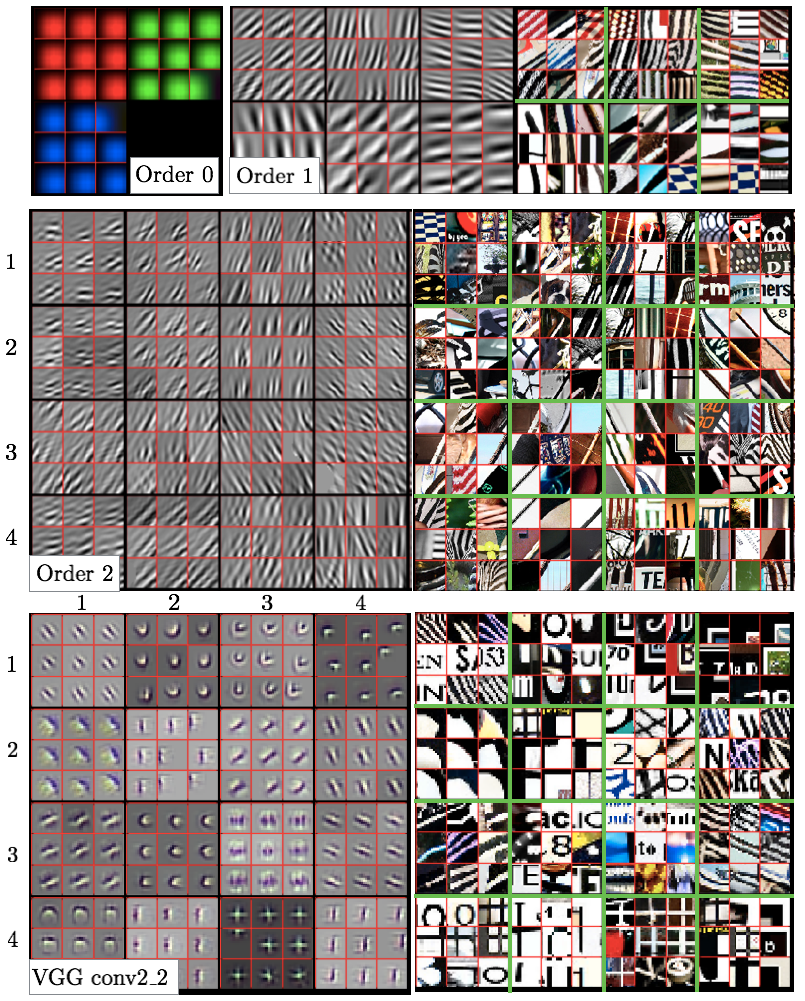
\includegraphics[width=1.1\textwidth]{\imgpath/deconv_images.png}}
      % \caption[Visualization of deconvolved features]
              % {Visualization of some deconvolved features.  9 coordinates are chosen in the
              % feature map for layer 1 $z^1$, 16 for the second layer
              % feature map $z^2$ and 16 for the third layer feature map.
              % The entire dataset is run, and 9 images that made the largest
              % activation at this point are noted. Deconvolution is then done on
              % the feature maps from these 9 images, and the results are shown
              % next to the actual images. Deeper layers are picking up more
              % complex structures. Taken from \cite{zeiler_visualizing_2014}.}
  % \end{figure}

